The training mode is an optional step which can be perfomed after the planning stage has been completed.
The training mode is dependant on the in the project case saved procedure steps.
While in training mode, information about the currently to be perfomed step is displayed inside the virtual operting room.
There, instructions, mainly about which procedure has to be performed, is shown.

\begin{figure}[h]
    \centering
    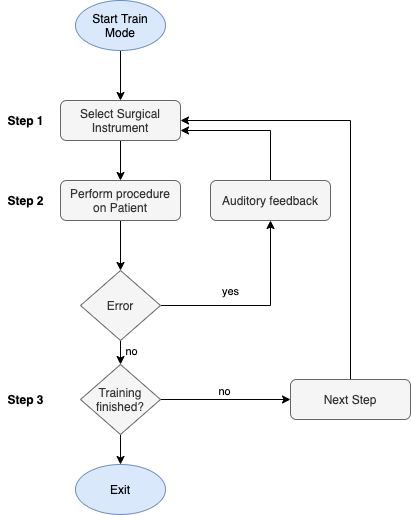
\includegraphics[width=225px]{images/implementation/features/training/training_flow.png}
    \caption{\label{fig::TrainingFlow}Simplistic Flow during Training Stage}
\end{figure}

The basic flow of interaction in this mode is depicted in Figure \ref{fig::TrainingFlow}.
\newline
\textbf{Step 1}: Users have to locate the correct surgical instrument and pick it up.
In case of the drilling or chiseling procedure, the correct attachment has to be chosen.

\begin{figure}
    \centering
    \begin{minipage}{.5\textwidth}
      \centering
      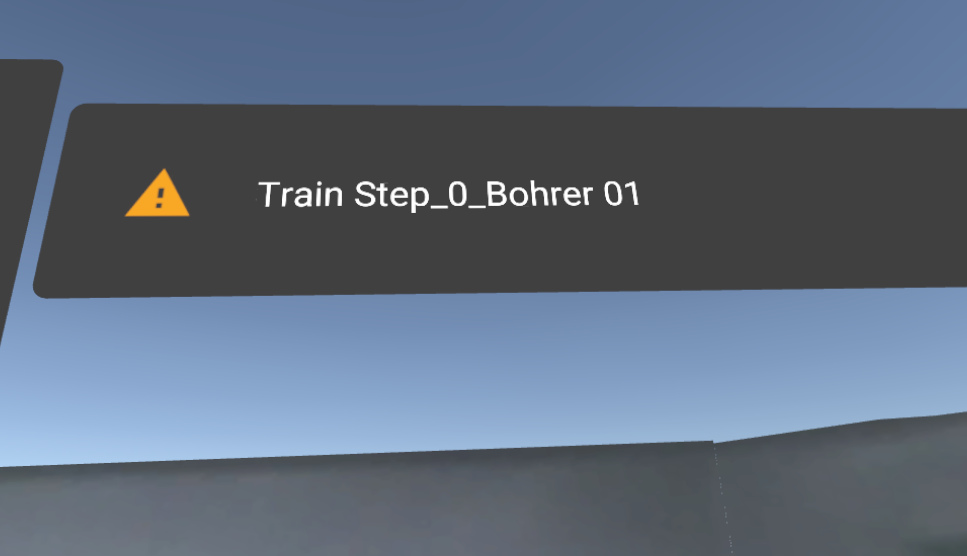
\includegraphics[width=0.95\linewidth]{images/implementation/features/training/train_guide.png}
    \end{minipage}%
    \begin{minipage}{.5\textwidth}
      \centering
      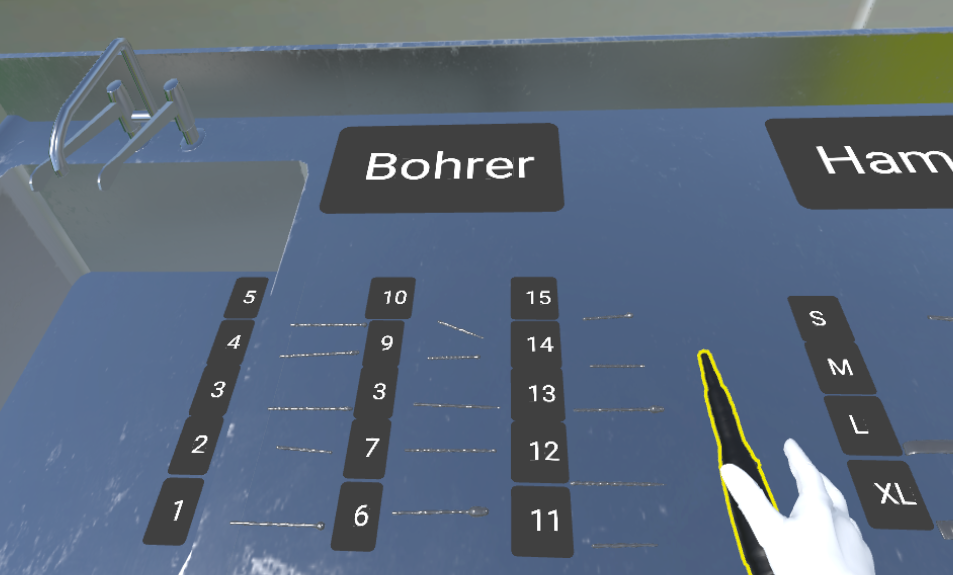
\includegraphics[width=0.915\linewidth]{images/implementation/features/training/train_select.png}
    \end{minipage}
    \begin{minipage}{1\textwidth}
        \centering
        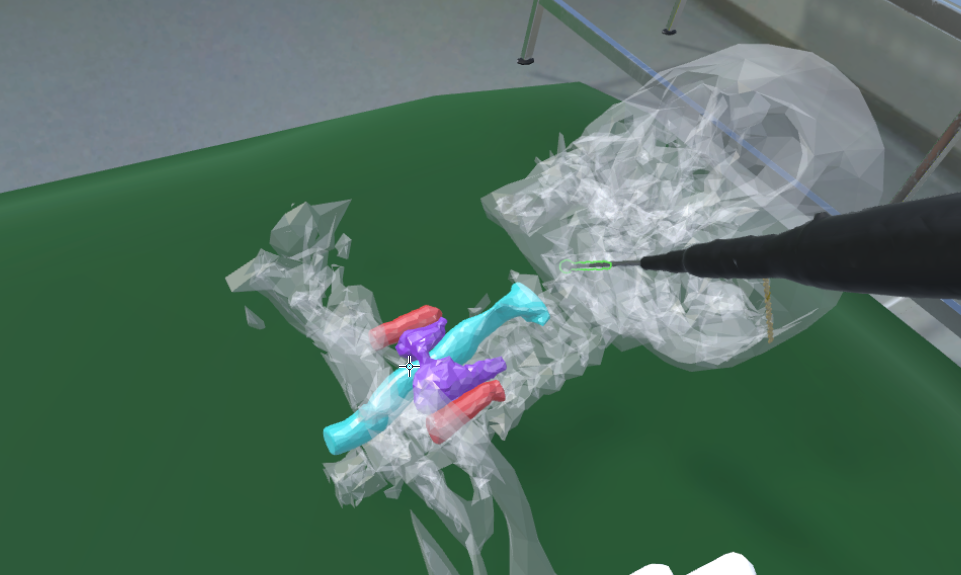
\includegraphics[width=0.95\linewidth]{images/implementation/features/training/training.png}
      \end{minipage}%
    \caption{\label{fig::TrainingMode}Training guidance and assistance}
  \end{figure}

\textbf{Step 2}: The current step which is to be perfomed will also be hinted at in the patients 3D model (Figure \ref{fig::TrainingMode}).
The outline of the current step is shown to the user, and the correct procedure has to be applied at the surgical site in which the outline is shown to progress.
If an error has been made (i.e. wrong attachment, wrong location), voice feedback is given and the user has to retry the procedure.
In the case of success, the voice feedback will signal that the next step is to be performed and the instructions and outline of the step will change accordingly.
\newline
\textbf{Step 3}: If all steps have been finished, the training mode will finish and the planning mode will resume.
